\renewcommand*\descriptionlabel[1]{\hspace\leftmargin$#1$}
\setcounter{tocdepth}{5}
\setcounter{secnumdepth}{5}
\newcommand{\minus}{\scalebox{0.65}[1.0]{$-$}}


\section{Molten Salt Reactors}

Modeling and simulation of liquid fueled molten salt reactors (MSRs) differs from solid fueled reactors in two main areas. The first is in the fresh fuel feed and fission product removal streams used during operation in MSRs, called online reprocessing. Modeling an MSR without online reprocessing will cause very different results during depletion calculations due to the lack of fresh fuel and buildup of fission products. In order to simulate this reprocessing functionality, software can either use batchwise reprocessing or continuous reprocessing.

The second difference is in the movement of the fuel salt, which causes delayed neutron precursors (DNPs) to move in the core. Because the DNPs have different decay times before the delayed neutrons are born, the effect of the fuel movement on each group varies. However, the overall result is more delayed neutrons in less important regions, such as external piping, which means there is a reduced effective delayed neutron fraction in the core.
%Modeling and simulation of liquid fueled molten salt reactors (MSRs) is different from modeling and simulation of solid fueled reactors in a few different areas. Two main areas of particular importance are the online reprocessing functionality and the movement of the fuel through the reactor. The online reprocessing functionality involves removing fission products from the fuel and adding fresh fuel during operation. The movement of the fuel causes a shift in the location of delayed neutron precursors (DNPs). In solid fueled reactors, the distribution of DNPs follows the flux profile, while in MSRs the DNPs move along with the fuel. This results in a reduction in the effective delayed neutron fraction due to decay of DNPs in less important regions.

\section{Online Reprocessing}

The online reprocessing functionality of MSRs is simulated in different ways depending on the particular software used, and depending on the methods employed by that software. The two main ways to approach the online reprocessing problem is by either using batch-wise reprocessing or continuous reprocessing. There are also different approaches in terms of modeling the full core and using a unit-cell model. 

%Codes implement batchwise reprocessing by running the simulation, stopping, and then adding and removing materials. The process is then iterated. This method is useful in that it is fairly straightforward to implement, can be calibrated to different removal efficiencies, and makes mass balancing of the core straightforward. Some issues with the batchwise approach are that using large time steps will make the results more inaccurate, it has increased computational cost with smaller time steps, and it is an approximation of the actual physical process of reprocessing. It is an approximation because, in online reprocessing of a reactor, the fission products are continuously removed while any feed flows are continuously fed into the reactor.
Codes such as SaltProc and older versions of ChemTriton implement batchwise reprocessing by running the simulation, stopping, and then adding and removing materials \cite{rykhlevskii_modeling_2019, betzler_molten_2017}. The process is then iterated. This method is useful because it is fairly straightforward to implement, easy to customize, and makes mass balancing of the core straightforward. Some issues with the batchwise approach are that using large time steps will make the results more inaccurate, it has increased computational cost with smaller time steps, it has to rerun each time step for pre-reprocessing and post-reprocessing, and it is an approximation of the actual physical process of reprocessing. It is an approximation because, in online reprocessing of a reactor, the fission products are continuously removed while any feed flows are continuously fed into the reactor.

%Continuous reprocessing is implemented by adding terms to the Bateman equation similar to an extra decay term. The benefits of using continuous reprocessing are that the model is physically accurate, it doesn't impact computational cost as much as a batchwise process, and it allows for large time steps to be used. A note should be made, however, that the time step size is still limited since the simulation will need to update based on the new material composition and evolving neutron spectrum. However, there is less error from inaccurate material removal and addition. The main downside of the continuous removal approach is that it is more cumbersome to implement and configure due to the nature of how it operates.
Codes such as Serpent2 and newer versions of ChemTriton implement continuous reprocessing by adding terms to the Bateman equation similar to an extra decay term, as can be seen in Equation (\ref{eq:Bateman_type_one_decay}) \cite{aufiero_extended_2013, jr_vicente_valdez_modeling_2020}. The benefits of using continuous reprocessing are that the model is more physically accurate, it doesn't impact computational cost as much as a batchwise process, and it allows for larger time steps to be used. However, the maximum time step size cannot become too large, or the simulation will become less accurate. This is because the neutron spectrum and cross section data does not update to the new material compositions until a new depletion step begins. 
%The main downsides of the continuous reprocessing approach are that it is more cumbersome to implement and difficult to configure due to the nature of how it operates.

Another aspect of online reprocessing that must be considered is mass balancing. For batchwise reprocessing, mass balancing can be solved in several different ways. One method is to have the net mass of the feed rate over some depletion step be equivalent to the mass removed over that same depletion step, which is the current approach used by SaltProc \cite{rykhlevskii_modeling_2019}. Alternatively, the volume of the system can be adjusted so that constant density is maintained in order to keep cross section data consistent \cite{ridley_method_2017}. Another approach is to move excess fuel salt into a bleed-off tank \cite{ridley_method_2017}. For continuous reprocessing, the depletion time steps can be much larger. This means that during the interval between steps, the mass will not be balanced. However, the same batchwise methods can be used with continuous reprocessing at new depletion steps. Implementing these approaches increases computational cost when performed in Serpent2. This is because using a single input script with depletion steps will cause each depeletion step to be run once, but altering the input script by changing volumes or removing mass to a bleed-off tank will cause the time step to be run twice.

\subsection{Batchwise Reprocessing}

%Imagine a process exists in which $X$\% of some element is removed from the fuel salt in the system over some time period T. For a batchwise approach, a straightforward approach would be to run the system, deplete for some time step $\tau$, remove $\gamma$\%, and repeat. The scaling term $\gamma$ for the removal efficiency is a linear approximation of the removal efficiency based on the time step adjustment and can be seen in Equation \ref{eq:batchwise_rem_eff}. An alternative approach is to establish a depletion time step $\tau$ such that the efficiency based time value $T$ is a multiple of $\tau$ and only have the batchwise removal occur at the steps when $\tau$ is a multiple of $T$. 

%\begin{equation} \hfill 
%\gamma = X \frac{\tau}{T}
%\hfill\label{eq:batchwise_rem_eff} \end{equation}
Batchwise reprocessing starts with some removal rate where $X$\% of some element is removed from the fuel salt in the system over some time period T. Over a depletion step $\tau$, $\gamma$\% of the element's mass is removed, where $\gamma$ corresponds to $X$ according to Equation (\ref{eq:batchwise_rem_eff}). The scaling term $\gamma$ for the removal efficiency is a linear approximation based on the time step adjustment in Equation (\ref{eq:batchwise_rem_eff}). If the time step used causes the removal fraction to be greater than 1, the amount removed remains at 100\% so as to not have negative mass.

An alternative approach is to establish a depletion time step $\tau$ such that the efficiency based time value $T$ is a multiple of $\tau$ and only have the $X\%$ batchwise removal occur at the steps when $\tau$ is a multiple of $T$, thus removing the need for scaling.

\begin{equation} \hfill 
\gamma = X \frac{\tau}{T}
\hfill\label{eq:batchwise_rem_eff} \end{equation}

For the Molten Salt Breeder Reactor (MSBR), SaltProc performs batchwise reprocessing every 3 days using a linear approximation of the cycle times given by Robertson in the ORNL report \cite{robertson_conceptual_1971, rykhlevskii_modeling_2019}. The xenon and krypton removals in SaltProc use a gas separation system equation, while the protactinium uses a modeled liquid-liquid reductive extraction process. These efficiencies differ from the cycle time values, causing slight differences in those terms. The MSBR also has two varying feed inputs of \ce{^{232}Th} and \ce{^{233}U}.

Examples of the batchwise method used in SaltProc can be seen in Equations \eqref{eq:SP_20s} and \eqref{eq:SP_60d}. Both examples show what the resulting mass removal per step, or $\gamma$, term should be for different cycle time values. The first shows a cycle time of 20s, which is shorter than the step time of 3 days. This results in a removal rate over 100\%, which is set to 100\%. The second shows a cycle time of 60 days, longer than the step size. This results in a 5\% removal per step. An alternative approach to the second example, which is implemented in the earlier versions of SaltProc, is to perform no removal until 60 days have elapsed and then remove 100\% of material.

\begin{equation} \hfill
X = 100\%, T = 20 s, \tau = 3 d \rightarrow \gamma > 100\% \rightarrow 100\% 
\hfill\label{eq:SP_20s} \end{equation}

\begin{equation} \hfill
X = 100\%, T = 60 d, \tau = 3 d \rightarrow \gamma = 5\%
\hfill\label{eq:SP_60d} \end{equation}

\subsection{Continuous Reprocessing}

%For a continuous approach, removing some fraction is dependent upon the particular isotope since the approach involves adding a term to the Bateman equation. This is one of the methods used in Serpent2 continuous reprocessing, where separations are only performed based on the element, not each particular isotope, an extension developed by Aufiero et al \cite{aufiero_extended_2013}. Equation \ref{eq:Bateman_default} shows the generic form of the Bateman equation, while Equation \ref{eq:Bateman_type_one_decay} shows the terms added to Equation \ref{eq:Bateman_default}, which are the reprocessing constants, or $\lambda_{r}$ added. 
The continuous approach manipulates the Bateman equation by adding a reprocessing term, which contains a reprocessing constant and the concentration of the isotope. This is one of the methods used in Serpent2 continuous reprocessing, an extension developed by Aufiero et al \cite{aufiero_extended_2013}. Equation (\ref{eq:Bateman_default}) shows the generic form of the Bateman equation, while Equation (\ref{eq:Bateman_type_one_decay}) shows the terms added to Equation (\ref{eq:Bateman_default}), which are the reprocessing constants, $\lambda_{r}$. These terms represent removal of the current isotope as well as feed of the current isotope from other sources.

\begin{equation} \hfill
\begin{split}
%\frac{dN}{dt} = \sum_j \lambda_j N_j + \gamma \Sigma_f \phi + \Sigma_k \phi - \lambda N - \Sigma \phi - C
\frac{dN_j}{dt}_{base} = \sum_{i \neq j}  & \left [ \left( \gamma_{i \rightarrow j} \sigma_{f, i} \Phi + \lambda _{i \rightarrow j} + \sigma_{i \rightarrow j} \Phi \right) N_i \right ]\\
 & - \left ( \lambda_j + \sigma_j \Phi \right ) N_j
\end{split}
\hfill\label{eq:Bateman_default} \end{equation}

\begin{equation} \hfill
%\frac{dN}{dt} = \sum_j \lambda_j N_j + \gamma \Sigma_f \phi + \Sigma_k \phi - \lambda N - \Sigma \phi - C
%\frac{dN_j}{dt} = \sum_{i \neq j} \left [ \left( \gamma_{i \rightarrow j} \sigma_{f, i} \Phi + \lambda _{i \rightarrow j} + \lambda _{reproc, i \rightarrow j} + \sigma_{i \rightarrow j} \Phi \right) N_i \right ] - \left ( \lambda_j + \lambda_{reproc, j} + \sigma_j \Phi \right ) N_j
%\frac{dN_j}{dt} = \sum_{i \neq j} \left [ \left( \gamma_{i \rightarrow j} \sigma_{f, i} \Phi + \lambda _{i \rightarrow j} + \lambda _{r, i \rightarrow j} + \sigma_{i \rightarrow j} \Phi \right) N_i \right ] - \left ( \lambda_j + \lambda_{r, j} + \sigma_j \Phi \right ) N_j + \sum_{mat} \lambda _{r, i \rightarrow j} N_i
\frac{dN_j}{dt}_{net} = \frac{dN_j}{dt}_{base} -  \lambda_{r, j} N_j + \sum_{mat} \lambda _{r, i \rightarrow j} N_i
\hfill\label{eq:Bateman_type_one_decay} \end{equation}

The symbols given in the equations are defined as follows from Equation \cite{leppanen_development_2007}:
\begin{description}
\item[N_j] is the atomic density of isotope j.
\item[\gamma_{i \rightarrow j}] is the fractional fission product yield of $j$ in the fission of isotope $i$.
\item[\sigma_{f, i}] is the microscopic fission cross section of isotope $i$.
\item[\Phi] is the spectrum-averaged scalar flux in the fuel region.
\item[\lambda _{i \rightarrow j}] is the decay constant of decay $i \rightarrow j$.
%\item[\lambda _{r, i \rightarrow j}] is the reprocessing constant for feed of $i \rightarrow j$ 
\item[\sigma_{i \rightarrow j}] is the microscopic transmution cross section of reaction $i \rightarrow j$.
\item[N_i] is the atomic density of isotope $i$.
\item[\lambda_j] is the decay constant of isotope $j$.
\item[\lambda_{r, j}] is the reprocessing constant for removal of isotope $j$.
\item[\sigma_j] is the microscopic total transmutation cross section of isotope $j$.
\item[\lambda _{r, i \rightarrow j}] is the reprocessing constant for feed of material $i \rightarrow j$.
\end{description}

%It can be seen visually that the reprocessing removal essentially operates as increasing the decay rate when applied in this manner. For example, increasing the decay rate of a particular element in a given material in Serpent2 also requires another material to gain a feed rate equivalent to that decay rate. The feed rate of a particular material is given by summing the removal rates of other materials for each isotope.
Equation \eqref{eq:Bateman_type_one_decay} shows that the reprocessing removal has the same mathematical operation as the decay rate. Unlike decay, the isotopes removed by reprocessing instead are transfered to a different material, which operates as a feed for that material. This can be seen in the summation term, which sums over the different materials and moves them from material $i$ to material $j$.

Serpent2 has three different settings for continuous reprocessing which alter the effect on the Bateman equations. The zeroth setting does not conserve mass, so it will not be discussed. The first setting, which adds a decay-like term to the Bateman equation, is shown in Equations (\ref{eq:Bateman_default}) and (\ref{eq:Bateman_type_one_decay}). This approach of adding a decay-like term to the Bateman equation has been done with other codes \cite{jr_vicente_valdez_modeling_2020, rodriguez-vieitez_transmutation_2002}. For this setting, three different approaches are implemented in order to compare their results.


The first approach is labeled the Cycle Time Decay (CTD) approach. It takes half the value of the cycle times and treats them as half life values. A similar method of treating removal periods for reprocessing can be seen in Brovchenko et al \cite{brovchenko_neutronic_2019}. Equation (\ref{eq:CTDex}) shows how this approach works with a cycle time of 20 seconds. The operation cuts the cycle time in half and then calculates the decay constant, or reprocessing constant, using the half life from the cycle time.

\begin{equation} \hfill
20s \rightarrow \tau = 10s \rightarrow \lambda_{r} = \frac{ln(2)}{\tau} \approx 6.93E\minus 2
\hfill\label{eq:CTDex} \end{equation}

The next approach is labeled the SaltProc Cycle Rate (SPCR) approach. It takes the same efficiency rates used by SaltProc, which uses 3 day depletion steps for the MSBR, and directly converts those rates to continuous reprocessing rates. Taking the inverse of the cycle time is a common way to generate the removal rate \cite{rykhlevskii_modeling_2019, nuttin_potential_2005}. Equation (\ref{eq:SPCRex}) shows how this approach works with a cycle time of 20s. This operation uses the SaltProc value, which in this case becomes 100\% removal over 3 days, converts it to be per second, and then converts that to the rate form usable in Serpent2.

\begin{equation} \hfill
20s \rightarrow \frac{1}{3 d} \rightarrow X = \frac{4E \minus 6}{1 s} \rightarrow \lambda_r = ln \left( \frac{1}{1 - X} \right) \approx 4E \minus 6
\hfill\label{eq:SPCRex} \end{equation}

This natural logarithm in this approach comes from the differential equation solution based on the removal rate provided. The method used to derive this equation can be seen in Equations \eqref{eq:nat_log_1}, \eqref{eq:nat_log_2}, and \eqref{eq:nat_log_3}. These equations assume that the $X$ term, or the fractional removal rate, is in units of per second.

\begin{equation} \hfill
\frac{dN}{dt} = -\lambda_r N
\hfill\label{eq:nat_log_1} \end{equation}

\begin{equation} \hfill
N(t) = (1-X) N_{cur} = N_{cur} e^{-\lambda_r}
\hfill\label{eq:nat_log_2} \end{equation}

\begin{equation} \hfill
-ln(1-X)  = \lambda_r = ln\left( \frac{1}{1-X} \right)
\hfill\label{eq:nat_log_3} \end{equation}

The final approach is labeled the Cycle Rate (CR) approach. It takes the cycle times and uses a linear approximation to generate the efficiency rate directly. Equation (\ref{eq:CRex}) shows how this approach works using a cycle time of 20 seconds. This operation takes the cycle time, determines the efficiency rate for 100\% removal over 20 seconds, and then uses that value to calculate the Serpent2 reprocessing constant.

\begin{equation} \hfill
20s \rightarrow X = \frac{1}{20 s} \rightarrow \lambda_r = ln \left( \frac{1}{1 - X} \right) \approx 5.12E\minus 2
\hfill\label{eq:CRex} \end{equation}

%Equations \ref{eq:Bateman_diff_removed} and \ref{eq:Bateman_X_removed} show the relationship between the net removal amount and the efficiency. Equations \ref{eq:Bateman_diff_control} through \ref{eq:Bateman_soln_control} show what the $\lambda$, or reprocessing constant, value would need to be set to such that, at the end of the simulation time $t_f$, the overall removal fraction is equal to $X$. These equations are a demonstration for a case in which there is no decay or production, only some initial amount that is removed continuously.

%\begin{equation} \hfill
%\frac{dN_{removed}}{dt} = \lambda N
%\hfill\label{eq:Bateman_diff_removed} \end{equation}

%\begin{equation} \hfill
%X = \frac{N_{removed}}{N_0 + N_{produced}}
%\hfill\label{eq:Bateman_X_precalc} \end{equation}


%\begin{equation} \hfill
%\frac{dN}{dt} = -\lambda N
%\hfill\label{eq:Bateman_diff_control} \end{equation}

%\begin{equation} \hfill 
%N(t) = N_0 e^{-\lambda t}
%\hfill\label{eq:Bateman_eqn_control} \end{equation}

%\begin{equation} \hfill
%X = \frac{N_{removed}}{N_0 + N_{produced}} = 1 - \frac{N_f}{N_0}
%\hfill\label{eq:Bateman_X_removed} \end{equation}

%\begin{equation} \hfill 
%\lambda = \frac{ln(\frac{1}{1-X})}{t_f}
%\hfill\label{eq:Bateman_soln_control} \end{equation}

%\begin{equation} \hfill 
%X = 1 - e^{-\lambda t_f}
%\hfill\label{eq:Bateman_soln_control} \end{equation}


%A different isotope which naturally decays with a decay constant of $\lambda_d$ will have a different set of equations, which can be seen in Equations \ref{eq:Bateman_diff_decay} through \ref{eq:Bateman_eqn_decay_X}. It can be seen that if a value of 0 is used in Equation \ref{eq:Bateman_eqn_decay_X} for the decay constant, then the value matches the result in Equation \ref{eq:Bateman_soln_control}.

%\begin{equation} \hfill
%\frac{dN}{dt} = -\lambda N - \lambda_d N
%\hfill\label{eq:Bateman_diff_decay} \end{equation}

%\begin{equation} \hfill 
%N(t) = N_0 e^{-(\lambda + \lambda_d) t}
%\hfill\label{eq:Bateman_eqn_decay} \end{equation}


%\begin{equation} \hfill
%\frac{dN_{removed}}{dt} = \lambda N = \lambda N_0 e^{-(\lambda + \lambda_d) t}
%\hfill\label{eq:Bateman_diff_decay_removed} \end{equation}

%\begin{equation} \hfill 
%N_{removed}(t) = \frac{\lambda N_0}{\lambda + \lambda_d} \left( 1 - e^{-(\lambda + \lambda_d) t} \right)
%\hfill\label{eq:Bateman_eqn_decay_removed} \end{equation}

%\begin{equation} \hfill 
%X = \frac{N_{removed}}{N_0 + N_{produced}} = \frac{\lambda}{\lambda + \lambda_d} \left( 1 - e^{-(\lambda + \lambda_d) t} \right)
%\hfill\label{eq:Bateman_eqn_decay_X} \end{equation}

%Although the results match when the decay is removed, while the decay is present, the results cannot be equivalent. This demonstrates one of the flaws of using continuous reprocessing, which is that the effects of the same reprocessing efficiency, $X$, on different isotopes of the same element requires unique reprocessing constants, $\lambda$, for each isotope in order for the removal efficiencies to be equivalent. Therefore, operating a continuous reprocessing scheme using a single removal constant for an element will fundamentally be non-physical due to the variances in removal efficiencies. The current system in Serpent2 allows for a removal constant to be applied to all isotopes of that element, which can circumvent this issue.

The second continuous reprocessing setting used in Serpent2 removes a constant value from each isotopic Bateman equation for an element. This approach can be seen in Equation \ref{eq:Bateman_diff_second_example}, where the $C$ term represents the constant value being removed by continuous reprocessing.

\begin{equation} \hfill
%\frac{dN}{dt} = \sum_j \lambda_j N_j + \gamma \Sigma_f \phi + \Sigma_k \phi - \lambda N - \Sigma \phi - C
\frac{dN_j}{dt} = \sum_{i \neq j} \left [ \left( \gamma_{i \rightarrow j} \sigma_{f, i} \Phi + \lambda _{i \rightarrow j} + \sigma_{i \rightarrow j} \Phi \right) N_i \right ] - \left ( \lambda_j + \sigma_j \Phi \right ) N_j - C
\hfill\label{eq:Bateman_diff_second_example} \end{equation}

This approach has flaws which can be directly demonstrated through an example. Imagine an element exists with two isotopes $A$ and $B$. There is a removal rate of 10\% per second defined for the element. A batchwise process could remove 10\% of each isotopes relative abundance after a second by using a one second time step, which is physical in terms of fractional removal. This can be seen directly in Table \ref{tab:cont_repr_appr}, where 10\% of both isotopes and the net count are removed.

\begin{table}[ht]
\renewcommand{\arraystretch}{1.25}
\caption{Serpent2 Second Setting Approaches}
\label{tab:cont_repr_appr}
\begin{center}
\begin{tabular}{ | c | c | c | c | c | c | c |}
 \hline
 Labels & Initial & Batch & Net & A & B & Null\\
 \hline
 \hline
 A & 1000 & 900 & 949.5 & 900 & 999 & 990\\
 B & 10 & 9 & -40.5 & -90 & 9 & 0\\
 \hline
 Net & 1010 & 909 & 909 & 810 & 1008 & 990 \\
 \hline
\end{tabular}
\end{center}
\end{table}

For the continuous reprocessing, the first attempt might be to try and remove 10\% of the net by splitting it amongst the isotopes evenly. The issue with this approach is immediately noticeable, which is that the concentration of isotope $B$ becomes negative, as can be seen in the $Net$ column. A logical next approach would be to try and make one of the isotopes exactly correct while bringing the other along with it, which can be seen in the $A$ and $B$ columns. The results of this approach are seen in the table, and it can be seen that only by looking at the isotope with the smallest concentration and using that to determine the amount to remove can the result be ensured to be non-negative. One final approach to consider is to set the smallest concentration to 0, and bring the other isotopes along. This approach can be seen in the $Null$ column, and it also does not work very well.

%Previously, this continuous reprocessing functionality in Serpent2 was undocumented, which led to difficulties in its usage by users \cite{rykhlevskii_modeling_2019}. Recently, however, the Serpent2 documentation was updated by this work as well as work performed at The University of Tennessee with Dr. Chvala and Alex Wheeler.

%Overall, it can be seen that in the two different approaches used in Serpent2, neither is able to maintain physicality like batchwise reprocessing does. However, different approximations can be used in order to apply the Serpent2 continuous reprocessing. Additionally, the way continuous reprocessing is applied can vary. Different uses could be using batchwise reprocessing for a fine mesh and continuous reprocessing for a coarse mesh, where the fine mesh is applied at beginning of cycle (BOC) and end of cycle (EOC) while the coarse mesh is used during steady-state (SS) operations. Another alternative is that the continuous reprocessing could be focused on certain isotopes, such as xenon-135, in order to allow for larger batchwise steps to be used.

\subsection{DNP Movement}

The movement of DNPs in liquid fueled molten salt reactors impacts the operation of the reactor directly by reducing the number of neutrons which are present in the important regions of the reactor \cite{wooten_review_2018}. In a solid fueled reactor, the flux and the concentration of delayed neutron precursors have the same profile. However, a moving fluid fuel causes the precursors to have a shifted profile based on the fluid flow rate, mixing, and decay rate of the precursors. This was shown very clearly by Jun Shi and Massimiliano Fratoni in their work, which can be seen in Figure \ref{fig:genfoam_dnp_locations}.

\begin{figure}[H]
  \centering
  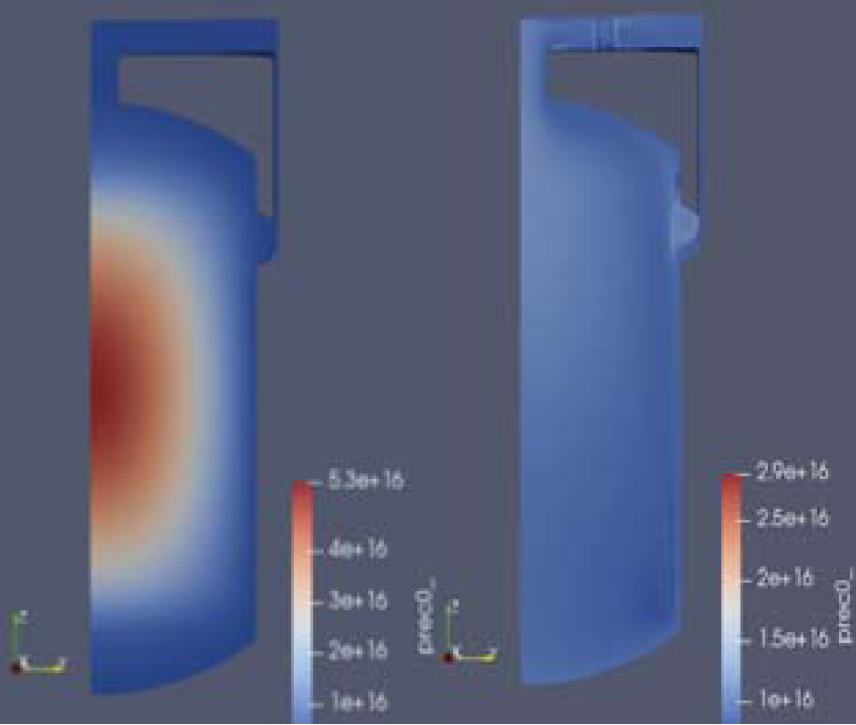
\includegraphics[scale=0.25]{images/dnp1.PNG}
  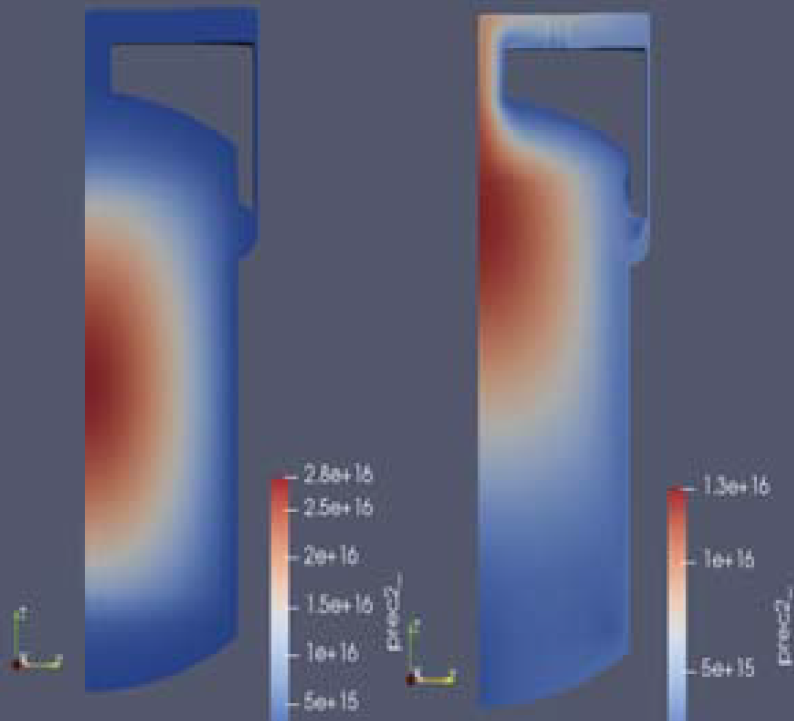
\includegraphics[scale=0.25]{images/dnp3.PNG}
  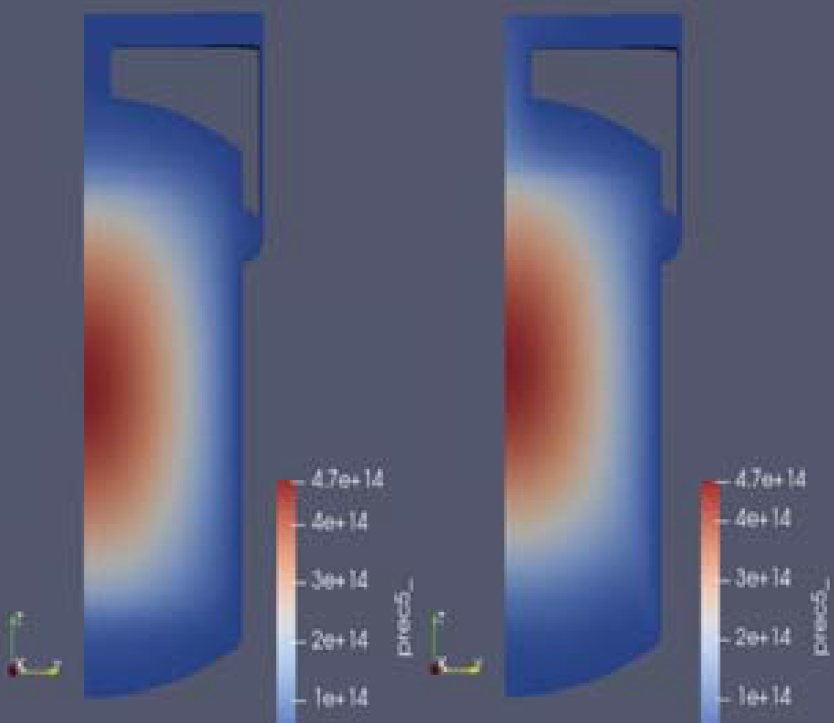
\includegraphics[scale=0.25]{images/dnp6.PNG}
  \caption{Plots of DNP concentrations in the molten salt reactor experiment \cite{shi_gen-foam_2021}. The left side of each image shows concentration with no flow, while the right shows the concentration with a 1200 gallon per minute flow rate. Top Left) Longest lived DNP group. Top Right) Third longest lived DNP group. Bottom) Shortest lived DNP group.}
   \label{fig:genfoam_dnp_locations}
\end{figure}

From these images, it can be seen that for the long shortest lived DNPs, the movement of the fuel does not have any significant impact upon the DNP distribution when compared to static fuel. This is reasonable since the precursors do not live for very long in this group, so they do not have much chance to travel. For the intermediate DNP group, there is a clear shift in the direction of the fuel flow, which causes more precursors to produce delayed neutrons in the less important piping  and upper plenum regions. The longest lived DNP group seems to be spread almost equally throughout the entire reactor, which means that those delayed neutrons are contributing significantly less to the overall neutron economy. Additionally, this reduces the overall effective delayed neutron fraction since the delayed neutrons are in less important regions. This directly affects the controllability of the reactor through the reactor period, which is heavily dependent upon the delayed neutrons.

\section{Depletion}

Depletion is the process of burning the fuel and simulating the changes to the materials this causes in the system. Depletion requires specific information to run properly, such as decay constants,  fission yields, and fission and transmutation cross section data. The fission and transmutation cross section data can come from a transport calculation, while the other data can be read from a data library \cite{leppanen_development_2007}. Additionally, running depletion involves solving the Bateman equations, a generic version of which can be seen in Equation \ref{eq:Bateman_default}.

There are several different approaches to solving these equations, such as the Transmutation Trajectory Analysis (TTA) method and the Chebyshev Rational Approximation Method (CRAM). These are the two different methods used in Serpent2, and are both built into Serpent2 \cite{leppanen_serpent_2015}. Other codes may use external software to compute depletion, such as REM used by MCNP and ORIGEN-S used by KENO-VI \cite{aufiero_extended_2013}. Another code, aside from Serpent2, that contains built-in depletion solvers is ERANOS \cite{aufiero_extended_2013}.

The purpose behind solving these equations and having depletion models is to generate an accurate representation of the composition of the target materials during reactor operation. This is important in determining how long the reactor can run, how the safety of the reactor develops over time, and how operation may have to change to adjust to the new reactor state. For molten salt reactors, depletion also allows for information regarding fresh fuel feed rate and fission product removal rates, as well as how variations of those parameters can affect reactor performance and behaviour.

\section{The Molten Salt Breeder Reactor}

The molten salt breeder reactor (MSBR) is a useful design to analyze for several reasons. Because it is a molten salt reactor, online reprocessing is used within the design. In addition, it contains an inner and outer zone, each of which has different neutronic behaviour \cite{robertson_conceptual_1971}. More specifically, the inner zone has a softer spectrum, a higher fission rate, and a 13\% fuel-to-graphite ratio \cite{park_whole_2015}. The outer zone has a harder spectrum, a higher breeding rate, and a 37\% fuel-to-graphite ratio. The inner and outer zones prove to be an issue when accurately modeling using a unit-cell or one-region approach, as those models are unable to capture the different characteristics of each region \cite{rykhlevskii_modeling_2019}. The differences in the regions can also be seen in Figure \ref{fig:msbr_ryklev}, which allows for the difference in the fuel-to-graphite ratio to be visually noticeable.

\begin{figure}[H]
  \centering
  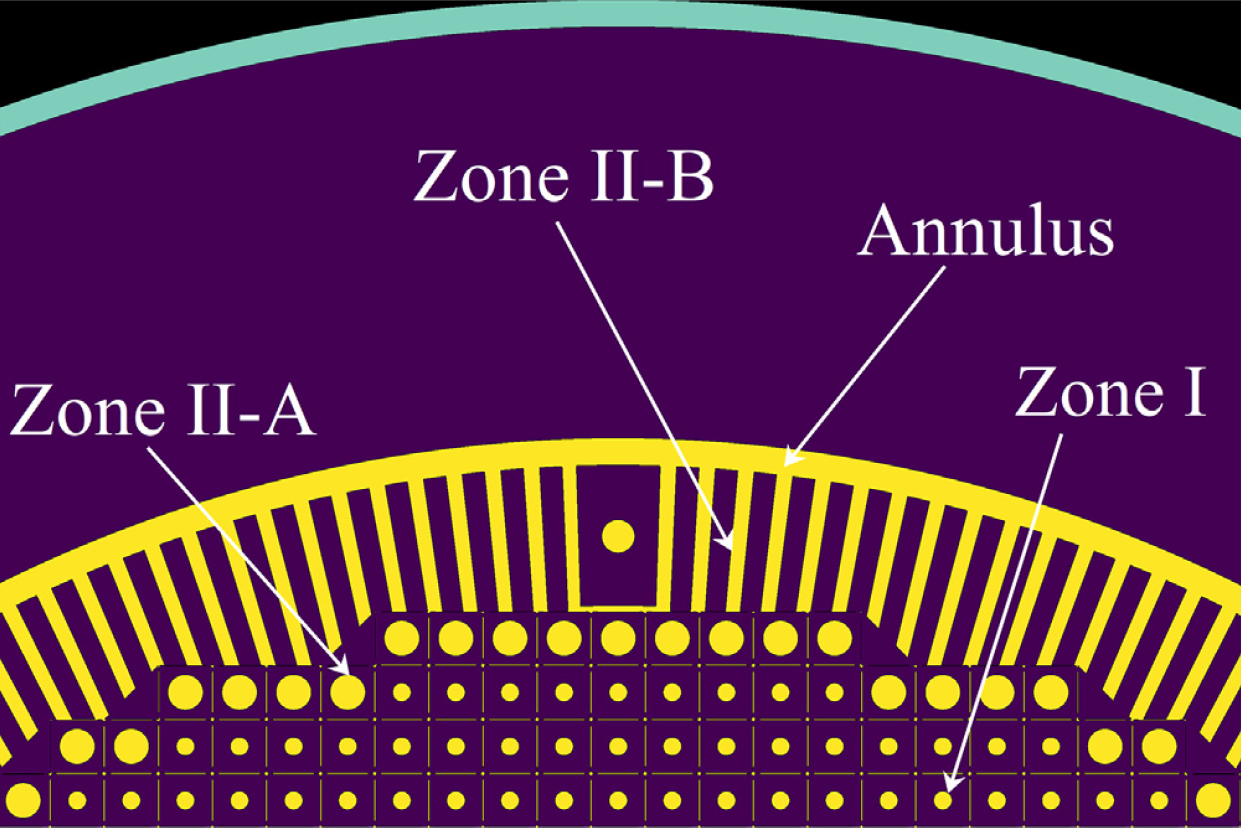
\includegraphics[scale=0.25]{images/msbr_ryk_1.PNG}
  \caption{MSBR core axial slice showing the different regions from \cite{rykhlevskii_modeling_2019}. Zones II-A and II-B are where the spectrum is harder and there is increased breeding. Zone I is where there is more fission and a softer spectrum. The yellow is fuel salt, the purple is graphite, and the cyan is the reactor vessel.}
   \label{fig:msbr_ryklev}
\end{figure}

For the online reprocessing aspect of the reactor, there are several mechanisms that contribute, as can be seen in Figure \ref{fig:msbr_robertson}. This figure shows how the reactor (1) links with the fuel salt pump (3), entrainment separator (14), and gas separator (13). The elements which are to be extracted, as well as their cycle times, are shown in Table \ref{tab:msbr_cycle_times}.


\begin{figure}[H]
  \centering
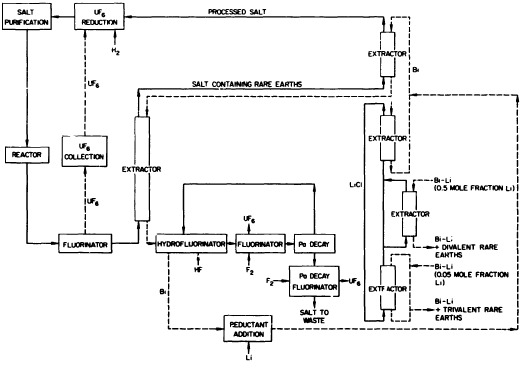
\includegraphics[scale=0.45]{images/msbr_flows_robertson.PNG}
  \caption{MSBR simplified flow diagram from \cite{robertson_conceptual_1971} showing part of primary side.}
   \label{fig:msbr_robertson}
\end{figure}

\begin{table}[H]
\renewcommand{\arraystretch}{1.25}
\caption{MSBR Online Reprocessing Cycle Times \cite{robertson_conceptual_1971}}
\label{tab:msbr_cycle_times}
\begin{center}
\begin{tabular}{ | p{0.27\linewidth} | p{0.25\linewidth} | p{0.35\linewidth} |}
 \hline
 Reprocessing Group & Element(s) & Cycle Time (Full Power)\\
 \hline
 \hline
 Rare Earths & Y, La, Ce, Pr, Nd, Pm, Sm, Gd & 50 days\\
 Rare Earths & Eu & 500 days\\
 Noble Metals  & Se, Nb, Mo, Tc, Ru, Rh, Pd, Ag, Sb, Te & 20 seconds\\
 Seminoble Metals & Zr, Cd, In, Sn &  200 days\\
 Gases & Kr, Xe & 20 seconds\\
 Volatile Fluorides & Br, I & 60 days\\
 Discard & Rb, Sr, Cs, Ba & 3435 days\\
 Salt Discard & Th, Li, Be, F & 3435 days\\
 Protactinium & Pa (233) & 3 days\\
 Higher Nuclides & Np (237), Pu (242) & 16 years\\
 \hline
\end{tabular}
\end{center}
\end{table}

From SaltProc's MSBR example, the removal of each group can be attributed to a particular process within the physical system \cite{rykhlevskii_modeling_2019}. The entrainment separator is used to remove the gases; a nickel mesh is used to remove noble metals, seminoble metals, and volatile fluorides; and various processes given by Robertson are lumped together into the liquid metal process which removes rare earths, discard, and protactinium \cite{robertson_conceptual_1971}. The higher nuclides are removed at such an infrequent rate that they are not included within the SaltProc processes. The MSBR design removes the protactinium with the intent that the protactinium-233 will not absorb neutrons and will instead be fed out of the core to decay into uranium-233, which can then be fed back into the core.


\section{MSR Modeling Approaches}

For modeling of MSRs, there are generally two different models which are used. The first is a model which takes a given fuel composition and analyzes the performance of the reactor given that fuel composition. This may include focus on DNP movement \cite{fei_molten_2020, shi_gen-foam_2021} or reactor dynamics \cite{singh_plant-level_2020, cervi_development_2019, aufiero_development_2014}.

The second type of model is one which depletes the fuel. Because the online reprocessing of an MSR has such large effects on its fuel composition, depletion models of MSRs typically incorporate online reprocessing. These models can also account for other factors, such as DNP movement, as shown by Zhou et al \cite{zhou_fuel_2018}. The movement of DNP can have a noticeable effect on reactor performance by affecting neutron energy spectra and distribution of delayed neutrons \cite{betzler_implementation_2017}. Most, however, focus primarily on depletion and do not consider the DNP movement during depletion, as can be seen in Table \ref{tab:codes_types}. In order to handle spatial dependence of fuel salt without modeling the piping of the core, models can use the scaled flux method \cite{betzler_liquid-fueled_2021}.

For all of the continuous reprocessing models given in Table \ref{tab:codes_types}, all of them use the "fictitious decay constant" approach, which is shown in Equation \eqref{eq:Bateman_type_one_decay}. For the batchwise models, they typically use the approach shown in Equation \eqref{eq:batchwise_rem_eff} and remove a fraction at each depletion step rather than bulk removal at certain steps.

%For modeling of MSRs, there are typically three main types of models which are used. The first is a model which takes a fuel composition and runs without accounting for reprocessing, but accounts for the fuel movement effects, such as DNP drift, shown by Fei et al \cite{fei_molten_2020}. The second is a model which accounts for both fuel movement and reprocessing, such as Zhou et al \cite{zhou_fuel_2018}. The third is a model which does not account for fuel movement but accounts for reprocessing. Models which use the second or third approach are detailed in Table \ref{tab:codes_types}.


% Remove scale and step columns from table, include in description of model
\begin{table}[H]
\renewcommand{\arraystretch}{1.25}
\caption{Molten Salt Reactor Models with Online Reprocessing}
\label{tab:codes_types}
\begin{center}
\begin{tabular}{ | c | c | c | c | c | c | c | c | }
 \hline
 Index & Reprocessing & Model & Reactor & DNP & Ref.\\
 \hline
 \hline
 1 & Batchwise & Full 3D & MSBR & No & \cite{rykhlevskii_modeling_2019}\\
 2 & Continuous & Full 3D & MSFR & No & \cite{aufiero_extended_2013}\\
 3 & Batchwise & Full 3D & MSBR & No & \cite{park_whole_2015}\\
 4 & Batchwise & Unit Cell & MSBR & No & \cite{betzler_molten_2017}\\
 \;\,4* & Continuous & Unit Cell & N/A & No & \cite{jr_vicente_valdez_modeling_2020}\\
 5 & Batchwise & Inf Lattice & DMSR & No &  \cite{ahmad_neutronics_2015}\\
 6 & Continuous & Full 3D & MSBR & Yes & \cite{zhou_fuel_2018}\\
 7 & Batchwise & Full 3D & MSBR & No & \cite{nuttin_potential_2005}\\
 8 & Batchwise & Full 3D & MOSART & No & \cite{sheu_depletion_2013}\\
 9 & Continuous & Inf Lattice & ADNA & No & \cite{rodriguez-vieitez_transmutation_2002}\\
 10 & Mixed & 2D Slice & MSFR & No & \cite{fiorina_preliminary_2012}\\
 11 & Continuous & Full 3D (?) & MSFR & No & \cite{zhuang_extended_2020}\\
 12 & Batchwise & Full 3D & Toy & No & \cite{ridley_method_2017}\\
 13 & Mixed & 2D Slice & N/A & Yes & \cite{h_f_bauman_rod_1971}\\
 14 & Mixed & Full 3D & TMSR & No & \cite{merle-lucotte_thorium_2007}\\
 \hline
\end{tabular}
\end{center}
\end{table}

The first entry in Table \ref{tab:codes_types} is SaltProc's MSBR example, which uses Serpent2, a full 3D core, 3 day time steps, and runs for 60 years. The batchwise reprocessing in SaltProc includes both the removal and feed processes.

The second entry is by Aufiero et al, and displays the Serpent2 newly developed continuous reprocessing functionality. A full 3D simplified core layout of the molten salt fast reactor (MSFR) is used, and continuous reprocessing is used to operate the removal and feed processes. It evaluates the model at various scales, from steady state uranium concentrations at over 60 years to radiotoxicity over $10^8$ years. The step sizes vary as well, though not specifically mentioned, appearing very small at BOC and expanding to around 10 years at SS for one of the figures presented.

The third entry by Park et al is very similar to the MSBR example in SaltProc, with the primary difference being MCNP6 is used for transportation calculations instead of Serpent2. The depletion was performed using CINDER90 and custom Python scripts. Another difference is that SaltProc uses adjusted values for the removal efficiency rates of xenon, krypton, and protactinium, while the work by Park et al uses the cycle time values from Robertson \cite{robertson_conceptual_1971}. This model uses 3 day time steps and models the fuel composition over 20 years.

The fourth entry is for ChemTriton, a tool designed for SCALE to perform online reprocessing of MSRs. It contains work on multiple reactors, such as the MSBR and the MSRE. The tool iteratively runs SCALE/TRITON over small time steps to simulate continuous reprocessing. For the MSBR case, 3 day time steps are used, similar to SaltProc and Park et al. The reason for not using shorter time steps is that using shorter time steps increases computational cost while also providing very little improvements to calculated eigenvalue and fuel cycle metrics, discussed by Betzler et al as well as by Powers et al \cite{powers_new_2013}.

ChemTriton has been updated after TRITON implemented new tools for continuous material feeds and removals. The work discusses in depth how the removal rates for isotopes can be calculated using a well mixed approximation and accounting for non-modeled piping by introducing a correcting decay factor. Although it does not account for DNP movement, it does account for neutron important regions without having to model the piping regions.

The fifth entry by Ahmad et al analyzes single fluid and two fluid denatured molten salt reactors (DMSRs). This work uses MCNP5 and ORIGEN2 as the codes to perform transport and depletion over 30 years. Although the steps at which fuel is adjusted is at 5 year intervals, the burnup intervals are actually set to 6 months. The reason such large steps were used is because the work analyzes proliferation and resource requirements for the reactors. This means that the neutronics and safety parameters were not as important, and so the model did not have to be as precise in that regard. Additionally, only gaseous fission products or fission products which are removed via sparging are included in the reprocessing scheme, no other chemical extraction takes place. This is because the authors wanted the system to be as simple as possible. ORIGEN provides continuous reprocessing capability, however for this work it would not have been necessary since the authors wanted to use a simpler approach for the model \cite{gauld_isotopic_2011}.

The sixth entry by Zhou et al is for FAMOS (Fuel cycle Analysis code for MOlten Salt reactors). This code uses OpenMC to generate homogenized cross section data followed by the DIF3D diffusion solver along with extensions to model DNP movement, thermal hydraulics, depletion, and continuous reprocessing. Their work also analyzes the molten salt fast reactor over 200 operational years. The depletion step size is not specifically given in the work, but from analysis of the plots, small time steps seem to have been used at the beginning of cycle and then larger time steps of ~100 days are then used for the rest of the steps.

The seventh entry by Nuttin et al analyzes the MSBR using a slightly simplified geometry with MCNP. The reprocessing approach used here is also the same as the approach used in SaltProc, which is to take the inverse of the cycle time to determine the removal rate. Depletion is performed in this work by coupling MCNP to an evolution program and the NJOY code. However, this work uses 10 day steps instead of 3 day steps that SaltProc uses. It also runs for 100 years instead of 20.

The eight entry by Sheu et al analyzes the Molten Salt Actinide Recycler \& Transmuter (MOSART) reactor and uses custom scripts to implement batchwise reprocessing. The codes used are SCALE6 for transport and TRITON for depletion. The step sizes used include 15, 30, and 60 days, in which the authors found that 30 days gave the best results in terms of accuracy and run time balancing for the 30 year simulation.

The ninth entry by Rodriguez-Vieitez analyzes the Accelerator-Driven Neutron Applications (ADNA) Tier-1 reactor using MCNP. Although the model used does implement continuous reprocessing in the Bateman equation, it is not used for the purpose of fuel cycle analysis and depletion. Rather, the work iteratively works towards the equilibrium fuel composition in order to analyze the effect of varying different reactor parameters, such as geometry.

The tenth entry by Fiorina et al is on the Molten Salt Fast Reactor (MSFR) and uses a modified version of the ERANOS-based EQL3D procedure. This model makes use of continuous reprocessing for non-soluble fission products, but uses batchwise reprocessing for soluble fission products. The batchwise reprocessing was incorporated for simplicity in the model. The time steps used are shorter at beginning of cycle at extend out to ~30 year steps for a 200 year depletion. Additionally, the radiotoxicity analysis extends out to 1 million years.

The eleventh entry by Zhuang et al discusses an OpenMC extension called OpenMCB-MSR to implement continuous reprocessing in an analysis of the MSFR. The depletion step sizes used are not specified in the work, though with continuous reprocessing step sizes could have been set to above single digit days and still maintained high precision.

The twelfth entry by Ridley and Chvala use batchwise reprocessing on a toy MSR using Serpent2 and a python library. The feed rates were set to fluctuate in order to maintain criticality while also accounting for density imbalance in Serpent2 by increasing the volume of the material. The full core 3D model was then analyzed using 7 day depletion steps for 10 years.

The thirteenth entry is on the Reactor Optimum Design (ROD) code, which allows users to use continuous or batchwise reprocessing for the MSR model. ROD operates by taking a one or two dimensional input and determining the equilibrium fuel composition. This is a useful code for determining a prediction of a model, but is less precise than more modern codes which offer more detailed geometry and other features.

The fourteenth entry by Merle-Lucotte et al covers depletion of the Thorium Molten Salt Reactor (TMSR) using MCNP4 \cite{goluoglu_software_1998} for transport and REM for material evolution. Continuous reprocessing is used for gaseous fission product extraction, while the other fission products are processed with batchwise reprocessing.

